\documentclass{article}


% if you need to pass options to natbib, use, e.g.:
%     \PassOptionsToPackage{numbers, compress}{natbib}
% before loading neurips_2023

% ready for submission
\usepackage[final]{neurips_2023}

% to avoid loading the natbib package, add option nonatbib:
%    \usepackage[nonatbib]{neurips_2023}


\usepackage[utf8]{inputenc} % allow utf-8 input
\usepackage[T1]{fontenc}    % use 8-bit T1 fonts
\usepackage{hyperref}       % hyperlinks
\usepackage{url}            % simple URL typesetting
\usepackage{booktabs}       % professional-quality tables
\usepackage{amsfonts}       % blackboard math symbols
\usepackage{nicefrac}       % compact symbols for 1/2, etc.
\usepackage{microtype}      % microtypography
\usepackage{xcolor}         % colors
\usepackage{graphicx}       % addtional package for show figures
\usepackage{amsmath}
\usepackage{float}

\title{MLPC 2025 Task 2: Data Exploration}


% The \author macro works with any number of authors. There are two commands
% used to separate the names and addresses of multiple authors: \And and \AND.
%
% Using \And between authors leaves it to LaTeX to determine where to break the
% lines. Using \AND forces a line break at that point. So, if LaTeX puts 3 of 4
% authors names on the first line, and the last on the second line, try using
% \AND instead of \And before the third author name.


\author{% 
  Team LABORER \AND
  Ali Doğukan Seven
  \And
  Yisong Tang
  \And 
  Karel Štícha
  \AND 
  Dmitrii Troitskii
}


\begin{document}


\maketitle


\begin{contributions}
  Ali Doğukan Seven was responsible for Parts 1 and 6. Karel Štícha wrote Part 2 and compiled the final report. Dmitrii Troitskii wrote Parts 3 and 4. Finally, Yisong Tang completed Part 5 and prepared the presentation.
\end{contributions}
%%%%%%%Part 1 Labeling Function%%%%%%%%%
\section{Labeling Function}
\subsection{Label Accuracy}
I verified the alignment between the labeling functions and the top 20 most popular keywords. As it turns out, they performed quite okay, with about 97\% of the pairs matching. In the remaining few cases of mismatch, the labels were still generally consistent with the category. The sounds mostly matched with the given timeframes, somewhat fitting into the mismatched ones, as I gave them a listen too. 

\subsection{Audio Features}
To identify which features were the most pertinent for classification discrimination, I used ANOVA F-scores. Top features included MFCC, embeddings, contrast, flatness, and bandwidth. These features seem to capture elements like pitch and texture of sounds, which come in handy for recognizing sound types. 

\subsection{Feature Clusters}
The higher-ranking features I gave are such sounds within a class tend to group quite nicely. The features thus help solidify a model in distinguishing types of sounds very well.
%%%%%%%Part 1 Labeling Function End%%%%%%%%%


%%%%%%%Part 2 Data Split%%%%%%%%%

\section{Data Split}

\subsection{Split Description}
To ensure reliable model training, meaningful hyperparameter tuning, and accurate evaluation, we divided our dataset into three distinct subsets: \textbf{a training set, a validation set, and a test set}. The training set, comprising 60\% of the data, was used to train the model. The validation set, which accounted for 20\%, served to tune the model’s hyperparameters and select the best-performing classifier. Lastly, the remaining 20\% formed the test set, which was used only once to estimate the final performance. 

\subsection{Information Leakage}
Information leakage occurs when information from outside the training dataset contributes to the training of the model. In our case, such leakage would occur from splitting the data at the frame level. Since consecutive frames are extracted from the same audio file, they are most likely very similar, splitting at the frame level could lead to frames from the same original recording being present in both the training and test sets. This would allow the model to learn patterns specific to individual recordings, resulting in inflated performance metrics and poor generalization. To avoid this, we performed the \textbf{data split at the file level}, ensuring that all frames from a specific audio file are assigned exclusively to a single dataset. As a result, the test data truly represent unseen input.  

\subsection{Obtaining Unbiased Performance Estimates}
To ensure an unbiased final performance estimate, we used the test set only for estimating the model’s performance. The training set was used solely for model fitting, while the validation set was used exclusively for tuning hyperparameters and model selection. This procedure prevents the model from being optimized for the test data and the final performance estimate reflect the model’s true ability to generalize on new, unseen data.

%%%%%%%Part 2 Data Split End%%%%%%%%%

\section{Audio Features}

\subsection{Selected Subset of Audio Features and Selection Process}

\textbf{Selected Features:}
\begin{itemize}
    \item \textbf{MFCC}: Mel-Frequency Cepstral Coefficients to capture timbral properties.
    \item \textbf{Embeddings}: Learned representations, possibly from a pretrained model.
    \item \textbf{Spectral Contrast}: Captures differences between spectral peaks and valleys.
    \item \textbf{Spectral Flatness}: Measures how noise-like a sound is.
    \item \textbf{Spectral Bandwidth}: Quantifies frequency spread.
    \item \textbf{Mel-Spectrogram}: A perceptually scaled time-frequency representation.
\end{itemize}

\textbf{Selection Process:}
\begin{itemize}
    \item \textbf{Feature Diversity}: Combined complementary features covering timbral, spectral, and perceptual aspects of audio.
    \item \textbf{Empirical Evaluation}: Features were loaded from precomputed `.npz` files and concatenated before dimensionality reduction.
    \item \textbf{Dimensionality Handling}: PCA was used to reduce feature size while preserving 95\% of the variance, which also helps prevent overfitting.
\end{itemize}

\subsection{Preprocessing Techniques Applied to Audio Features}

\textbf{Preprocessing Steps:}
\begin{itemize}
    \item \textbf{Standardization}: All features were normalized using \texttt{StandardScaler} to have zero mean and unit variance.
    \item \textbf{Dimensionality Reduction}: Principal Component Analysis (PCA) was applied to compress features while retaining 95\% of total variance.
    \item \textbf{Batch Transformation}: The same pipeline was fitted on the training set and then applied to validation and test sets to ensure consistency.
\end{itemize}


\section{Evaluation}

\subsection{Evaluation Criterion for Comparing Hyperparameter Settings and Algorithms}

\textbf{Chosen Criterion:}
\begin{itemize}
    \item \textbf{F1-Score (Macro-Averaged)}: This metric was used to evaluate and compare model performance. It calculates the F1-score for each class independently and then averages them, ensuring that rare and frequent classes are treated equally.
\end{itemize}

\textbf{Rationale:}
\begin{itemize}
    \item \textbf{Class Imbalance}: Many of the sound events occur infrequently, so metrics like accuracy would not reflect true performance.
    \item \textbf{Balanced Trade-off}: Macro-F1 balances both false positives and false negatives, which is important for multi-label tasks.
    \item \textbf{Cross-Validation Integration}: The F1-score was directly used as the scoring function during hyperparameter tuning via \texttt{GridSearchCV}.
\end{itemize}

\subsection{Baseline and Best Possible Performance}

\textbf{Baseline Performance:}
\begin{itemize}
    \item \textbf{Definition}: The baseline is defined by a naive model that always predicts the absence of events (all-zero labels).
    \item \textbf{Computation}: Based on the mean positive rate of the validation set across all classes, the baseline accuracy is approximately \( 1 - \text{mean positive rate} \).
    \item \textbf{Purpose}: This baseline reflects how well a model could perform by simply exploiting class imbalance — without learning meaningful patterns.
\end{itemize}

\textbf{Best Possible Performance:}
\begin{itemize}
    \item \textbf{Definition}: The best performance corresponds to the highest macro F1-score obtained through model selection and tuning.
    \item \textbf{Estimation}: This was achieved via \texttt{GridSearchCV} and cross-validation, using various models and hyperparameters. While perfect classification is unlikely due to label noise and overlapping events, the best model significantly outperforms the baseline.
\end{itemize}

\section{Experiments}

\subsection{Linear SVM}
\begin{itemize}
  \item \textbf{Hyperparameter:} Regularization coefficient $C \in \{0.01, 0.1, 1, 10, 100\}$.
  \item \textbf{Performance Curve:} Training F1 $\approx0.7787$, Validation F1 $\approx0.7747$ remain stable across $C$.
  \item \textbf{Over- vs.\ Under-fitting:} Train F1 $\approx$ Val F1, both well below 1.0 $\rightarrow$ slight under-fitting; no over-fitting observed.
  \item \textbf{Conclusion:} $C=1$ offers a good trade-off; further tuning yields no significant gain.
\end{itemize}

\subsection{Decision Tree}
\begin{itemize}
  \item \textbf{Hyperparameter:} Maximum depth $\text{max\_depth} \in \{5, 10, 15, 20, \text{None}\}$.
  \item \textbf{Performance Curve:}
    \begin{itemize}
      \item $\text{depth}=5$: Train/Val F1 $\approx0.65$ (under-fitting).
      \item $\text{depth}=10$: Best validation F1 $\approx0.674$ (Train $\approx0.807$).
      \item $\text{depth}>10$: Train F1 increases, Val F1 decreases (over-fitting).
    \end{itemize}
  \item \textbf{Over- vs.\ Under-fitting:} Depth $<10$ under-fits; depth $>10$ over-fits.
  \item \textbf{Conclusion:} Optimal depth $=10$; deeper trees memorize noise and degrade generalization.
\end{itemize}

\subsection{SGDClassifier (Logistic Regression)}
\begin{itemize}
  \item \textbf{Hyperparameter:} L2 regularization strength $\alpha \in \{10^{-6},10^{-5},10^{-4},10^{-3},10^{-2},10^{-1}\}$.
  \item \textbf{Performance Curve:}
    \begin{itemize}
      \item $\alpha=10^{-5}$: Best Train F1 $\approx0.7483$, Val F1 $\approx0.7480$.
      \item $\alpha\ge10^{-4}$: Both F1 scores drop (under-fitting).
      \item $\alpha=10^{-6}$: Train F1 $>$ Val F1 (slight over-fitting).
    \end{itemize}
  \item \textbf{Over- vs.\ Under-fitting:} \(\alpha\gg10^{-5}\) under-fits; \(\alpha\ll10^{-5}\) over-fits.
  \item \textbf{Conclusion:} $\alpha=10^{-5}$ balances bias and variance well.
\end{itemize}

\begin{figure}[h]
  \centering
  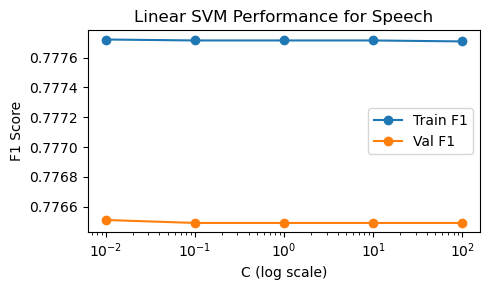
\includegraphics[width=0.3\linewidth]{figs_tang/svm.png}
  \hfill
  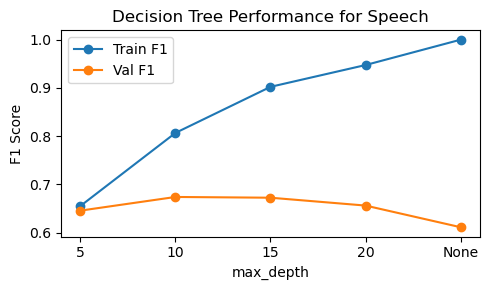
\includegraphics[width=0.3\linewidth]{figs_tang/dt.png}
  \hfill
  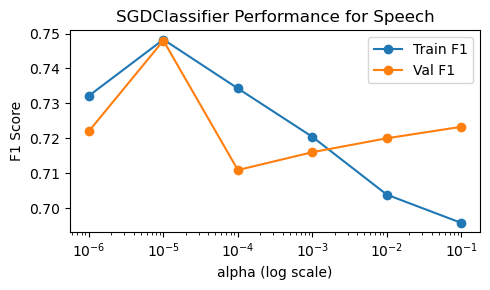
\includegraphics[width=0.3\linewidth]{figs_tang/sgd.png}
  \caption{Performance curves for Linear SVM (left), Decision Tree (middle), and SGDClassifier (right).}
  \label{fig:hp_curves}
\end{figure}

\subsection{Model Comparison}
\begin{table}[h]
\centering
\begin{tabular}{lccc}
\toprule
\textbf{Model} & \textbf{Best Hyperparameter} & \textbf{Validation F1} & \textbf{Avg Training Speed} \\
\midrule
Linear SVM     & $C=1$                        & 0.7748                & 44 s/class             \\
SGDClassifier  & $\alpha=10^{-5}$             & 0.7480                & 5–90 s/class            \\
Decision Tree  & max\_depth=10                & 0.6741                & 438 s/class             \\
\bottomrule
\end{tabular}
\caption{Comparison of the three classifiers on the validation set.}
\end{table}

\subsection{Final Model Performance}
The selected model (Linear SVM with $C=1$) was evaluated on the held-out test set using six features.
The overall Macro-F1 score across 58 classes is \textbf{0.5381}, reflecting average performance on frequent and rare classes.

\section{Analysing Predictions}

\subsection{File: 451475}
The model is weak in detecting some sounds while multiple events interfere. Between 00:05 and 00:08, speech is present but considered not recognized because of its lower volume. From 00:10 to 00:13, loud jackhammer sounds drown exchange horn honks-another sound.

It appears that the model tends to ignore those sounds that are quieter when there is a louder sound. There are sounds that humans simply have difficulty telling apart (e.g., jackhammer vs hammer), and some of this misclassification may be down to this.

\subsection{File: 27157}
There is much confusion here between speech and motor sounds. The Motor sounds may have similar waveforms to speech. Background noise could be the reason for this. The model perceives indistinct or low-pitched speech as sounds of engines or motor-sounds.

\subsection{Conclusion}
The classifier has problems with overlapping events and similar acoustic classes. Improvement might be possible with some postprocessing, e.g., averaging predictions over time or filtering out frames with low confidence.



\end{document}